
\section{Probabilistic label trees}
\label{app:plt}

An example of a probabilistic label tree (\Algo{PLT}) for 4 labels $(y_1,y_2,y_3,y_4)$ is given in Fig.~\ref{fig:plt}. To estimate posterior probability $\eta(\bx, j) = \prob(y_j = 1 \given \bx)$, \Algo{PLT} uses a path from a root to the $j$-th leaf.
In each node $t$, we associate with a training instance $(\bx,\by)$ a label $z_t$ such that:
$$
z_t = \assert{\textstyle \sum_{j \in L(t)} y_j \ge 1} \quad \textrm{(or equivalently $z_t = \bigvee_{j \in L(t)} y_j$)}
$$
Recall that $L(t)$ is a set of all leaves of a subtree with the root in the $t$-th node. In leaf nodes the labels $z_j$, $j \in L$, correspond to original labels $y_j$.
%
\begin{figure}[h]
	\begin{center}
		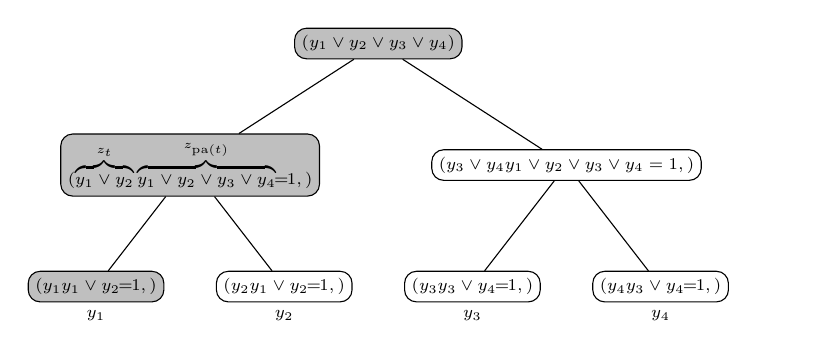
\begin{tikzpicture}[scale = 0.85,every node/.style={scale=0.85},
		regnode/.style={circle,draw,minimum width=1.5ex,inner sep=0pt},
		leaf/.style={circle,fill=black,draw,minimum width=1.5ex,inner sep=0pt},
		pleaf/.style={rectangle,rounded corners=1ex,draw,font=\scriptsize,inner sep=3pt},
		pnode/.style={rectangle,rounded corners=1ex,draw,font=\scriptsize,inner sep=3pt},
		rootnode/.style={rectangle,rounded corners=1ex,draw,font=\scriptsize,inner sep=3pt},
		activerootnode/.style={rectangle,rounded corners=1ex,draw,font=\scriptsize,inner sep=3pt,line width=1pt},
		activenode/.style={rectangle,rounded corners=1ex,draw,font=\scriptsize,inner sep=3pt,line width=1pt},
		activepleaf/.style={rectangle,rounded corners=1ex,draw,font=\scriptsize,inner sep=3pt,line width=1pt},
		level/.style={sibling distance=16em/#1, level distance=12ex}
		]
		\node (z) [rootnode,fill=lightgray] {\thickmuskip=-1.5mu $\prob(y_1\lor y_2 \lor y_3 \lor y_4 \given\bx)$}
		child {node (a) [pnode,fill=lightgray] {\thickmuskip=-1.5mu $\prob(\overbrace{y_1 \lor y_2}^{z_t}\given \overbrace{y_1 \lor y_2 \lor y_3  \lor y_4}^{z_{\mathrm{pa}(t)}}=1, \bx)$} 
			child {node [label=below:{ \scriptsize \thickmuskip=-1.5mu $y_1$}] (b) [pleaf,fill=lightgray] {\thickmuskip=-1.5mu $\prob(y_1\given y_1 \lor y_2=1, \bx)$} edge from parent node[above left]{}}
			child {node [label=below:{\scriptsize \thickmuskip=0mu $y_2$}] (g) [pleaf] {\thickmuskip=-1.5mu $\prob(y_2\given y_1 \lor y_2 = 1, \bx)$} edge from parent node[above right]{}}
			edge from parent node[above left]{}
		}
		child {node (j) [pnode] {$\prob(y_3 \lor y_4 \given y_1 \lor y_2 \lor y_3 \lor y_4 = 1, \bx)$}
			child {node [label=below:{ \scriptsize \thickmuskip=0mu $y_3$}] (k) [pleaf] {\thickmuskip=-1.5mu $\prob(y_3\given y_3 \lor y_4 = 1, \bx)$} edge from parent node[above left]{}}
			child {node [label=below:{ \scriptsize \thickmuskip=0mu $y_4$}] (l) [pleaf] {\thickmuskip=-1.5mu $\prob(y_4\given y_3 \lor y_4 = 1,  \bx)$}
				{
					child [grow=right] {node (s) {} edge from parent[draw=none]
						child [grow=up] {node (t) {} edge from parent[draw=none]
							child [grow=up] {node (u) {} edge from parent[draw=none]}
						}
					}
				}
				edge from parent node[above right]{}
			}
			edge from parent node[above right]{}
		};
		\end{tikzpicture}
\end{center}
\caption{An example of a probabilistic label tree for 4 labels $(y_1,y_2,y_3,y_4)$.}
\label{fig:plt}
\end{figure}
%

Consider the leaf node $j$ and the path from the root to this leaf node. Using the chain rule of probability, we can express $\eta(\bx, j)$ in the following way:
\begin{equation}
\eta(\bx, j) = \prod_{t \in \Path{j}} \eta_T(\bx, t)\,,
\label{eqn:probabilistic_tree_appendix}
\end{equation}
where $\eta_T(\bx, t) = \prob(z_t = 1 \given z_{\pa{t}} =1, \bx)$, for all non-root nodes $t$, and $\eta(\bx, t) = \prob(z_t = 1 \given \bx)$, if $t$ is the root node (denoted by $r(T)$). 

To see the correctness of (\ref{eqn:probabilistic_tree_appendix}) notice that $z_{t} = 1$ implies $z_{\pa{t}} = 1$. So, for non-root nodes $t$ and $\pa{t}$ we have:
\begin{eqnarray*}
\eta_T(\bx,t) \eta_T(\bx, \pa{t}) & = &  \prob(z_t = 1 \given z_{\pa{t}} =1, \bx)\prob(z_{\pa{t}} = 1 \given z_{\pa{\pa{t}}} =1, \bx)\\
& = & \frac{\prob(z_t = 1 , z_{\pa{t}} =1, \bx)}{\prob(z_{\pa{t}} =1, \bx)} \frac{\prob(z_{\pa{t}} = 1, z_{\pa{\pa{t}}} =1, \bx)}{\prob(z_{\pa{\pa{t}}} =1, \bx)} \\
& = & \frac{\prob(z_t = 1, \bx)}{\prob(z_{\pa{t}} =1, \bx)} \frac{\prob(z_{\pa{t}} = 1, \bx)}{\prob(z_{\pa{\pa{t}}} =1, \bx)} \\
& = & \frac{\prob(z_t = 1, \bx)}{\prob(z_{\pa{\pa{t}}} =1, \bx)} \,.
\end{eqnarray*}
In words, the probability associated with the parent node $\pa{t}$ cancels out and we can express $\eta_T(\bx,t) \eta_T(\bx, \pa{t})$ as the product of probabilities associated only with node $t$ and its grandparent node $\pa{\pa{t}}$. 
%
Applying the above rule consecutively to $\prod_{t \in \Path{j}} \eta_T(\bx, t)$ and recalling that for the root note $\eta_T(\bx, r(T)) = \prob(z_{r(T)} = 1 \given \bx)$, we finally get $\eta(\bx, j)$. 

Below we show that \Algo{PLT}s posses strong theoretical guarantees. We derive a relation between  estimation error minimized by the node classifiers and estimation error of posterior probabilities $\eta(\bx,j)$. This relation states that we can upperbound the latter error by the former. This also implies that for optimal node classifiers we get optimal multi-label classifier in terms of estimation of posterior probabilities.


We are interested in bounding the estimation error of posterior probabilities of labels at point $\bx$
$$
\ell(\eta(\bx),\heta(\bx)) = \frac{1}{m} \sum_{j=1}^m |\eta(\bx, j) - \heta(\bx, j)| \,,
$$
in terms of an estimation error of node classifiers
$$
\ell(\eta_T(\bx, t), \heta_T(\bx, t)) = |\eta_T(\bx, t) - \heta_T(\bx, t)  | \,.
$$

Expressing $\eta(\bx, j)$  and $\heta(\bx, j)$ by (\ref{eqn:probabilistic_tree_appendix}) and applying Lemma~2 from~\cite{Beygelzimer_et_al_2009b}, we get:
\begin{equation}
\left | \eta(\bx, j) - \heta(\bx, j) \right | \le \sum_{t \in \Path{j}} \left | \eta_T(\bx, t) - \heta_T(\bx, t) \right | \,.
\label{eqn:estimation_bound}
\end{equation}

Equation (\ref{eqn:estimation_bound}) already shows that minimization of the estimation error by node classifiers improves the overall performance of \Algo{PLT}s. We can show, however, even a more general result concerning surrogate regret bounds by referring to the theory of  strongly proper composite losses~\cite{Agarwal_2014}. 

Assume that a node classifier has a form of a real-valued function $f_t$. Moreover, there exists a strictly increasing (and therefore invertible) link function $\psi: [0,1] \rightarrow \mathbb{R}$ such that $f_t(\bx) = \psi(\heta_T(\bx,t))$. Recall that the regret of $f_t$ in terms of a loss function $\ell$ at point $\bx$ is defined as:
$$
\reg_{\ell}(f_t \given \bx) = L_{\ell}(f_t \given \bx) - L_{\ell}^*(\bx) \,,
$$
where $L_{\ell}(f_t \given \bx)$ is the expected loss  at  point $\bx$:
$$
L_{\ell}(f \given \bx) = \mathbb{E}_{y_j\given\bx} \left [ \ell  (y_j, f_t(\bx)) \right ] \,,
$$
and  $L_{\ell}^*(\bx)$ is the minimum expected loss at point $\bx$.

If a node classifier is trained by a learning algorithm that minimizes a strongly proper composite loss, e.g.,  squared, exponential, or logistic loss, like in our implementation (see in Appendix \ref{sec:training_of_node_classifiers}), then the bound (\ref{eqn:estimation_bound}) can be expressed in terms of the regret of this loss function: 
$$
\left | \eta_T(\bx, t) - \psi^{-1}(f_t)  \right | \le \sqrt{ \frac{2}{\lambda}} \sqrt{\reg_\ell(f_t \given \bx)}
$$
where $\lambda$ is a strong properness constant specific for a given loss function (for more detail, see~\cite{Agarwal_2014}). By putting the above inequality into~(\ref{eqn:estimation_bound}), we get
$$
\left | \eta(\bx, j) - \heta(\bx, j) \right | \le \! \sum_{t \in \Path{j}} \! \left | \eta_T(\bx, t) - \heta_T(\bx, t) \right | = \!  \sum_{t \in \Path{j}}  \! \left | \eta_T(\bx, t) - \psi^{-1}(f_t)  \right | \le  \! \sum_{t \in \Path{j}}  \! \sqrt{ \frac{2}{\lambda}} \sqrt{\reg_\ell(f_t \given \bx)}
$$ 


%Consider the label-wise KL-divergence between true posterior probabilities $\eta(\bx, j)$ and their estimates $\heta(\bx, j)$:
%$$
%\KLD(\eta(\bx) || \heta(\bx)) = \frac{1}{m}\sum_{j=1}^m \KLD(\eta(\bx,j) || \heta(\bx,j)) = \frac{1}{m}\sum_{j=1}^m \left ( \eta(\bx,j) \log \frac{\eta(\bx,j)}{\heta(\bx,j)} + (1 -\eta(\bx,j)) \log \frac{1- \eta(\bx,j)}{1 - \heta(\bx,j)}\right ) 
%$$
%Let us remark that $\KLD(\eta(\bx,j) || \heta(\bx,j))$  is equivalent to the conditional logistic regret defined as:
%$$
%\reglog(\heta(\bx,j) \given \bx) = L_{\log}(\heta(\bx,j) \given \bx) - L_{\log}^*(\bx) \,,
%$$
%where $L_{\log}(\heta(\bx,j) \given \bx)$ is the expected logistic risk at  point $\bx$:
%$$
%L_{\log}(\heta(\bx,j) \given \bx) = \mathbb{E}_{y_j\given\bx} \ell_{\log} (y_j, \heta(\bx,j)) = \mathbb{E}_{y_j\given\bx} \left ( y_j \log \heta(\bx,j) + (1 - y_j) \log (1 - \heta(\bx,j)) \right ) \,.
%$$
%and  $L_{\log}^*(\bx)$ is the minimum logistic risk at point $\bx$ achieved by $\heta(\bx,j) = \eta(\bx,j)$. %as says a standard result on the theory of proper losses (see, e.g., \citep{Reid_Williamson_2010}).
%
%Because of (\ref{eqn:probabilistic_tree_appendix}), we can rewrite the above to:
%$$
%\KLD(\eta || \heta) = \frac{1}{m}\sum_{j=1}^m \left (  \prod_{t \in \Path{j}} \eta_T(\bx, t)\log \frac{ \prod_{t \in \Path{j}} \eta_T(\bx, t)}{\ \prod_{t \in \Path{j}} \heta_T(\bx, t)} + (1 - \prod_{t \in \Path{j}} \eta_T(\bx, t)) \log \frac{1-  \prod_{t \in \Path{j}} \eta_T(\bx, t)}{1 -  \prod_{t \in \Path{j}} \heta_T(\bx, t)}\right ) 
%$$

\section{Training of node classifiers}
\label{sec:training_of_node_classifiers}

In each node $t$ we trained a linear classifier $f_t(\bx) = \bw \cdot \bx$, where $\bx = (1, x_1, \ldots, x_p)$.  To this end we used a variant of stochastic gradient descent to minimize logistic loss. Albeit successfully used in large scale learning, the optimization of empirical loss using stochastic gradient descent is a particularly challenging task when the number of features and labels is large. The step function should ensure a quick convergence in order to reduce the number of required training epochs. Furthermore, it should support sparse updates of the weights (i.e., only weights for non-zero features should be updated to ensure fast training time). % and auxiliary data structures. 
\citet{Duchi_Singer_2009} propose a two phase gradient step:
\begin{align*}
	\label{eq:fobos}
	\bm{w}_{t+\frac12} &= \bm{w}_t - \gamma_t \bm{g}_t\\
	\bm{w}_{t+1} &= \argmin_{\bm{w}}\left\{ \frac12 \norm[\big]{ \bm{w} - \bm{w}_{t+\frac12}}^2
	+ \lambda \gamma_{t} r(\bm{w})\right\}
\end{align*}
where $\bm{w}_t$ is the weight vector at time step $t$, $r(\bm{w})$ is a
regularization function, $\lambda$ is regularization parameter, and $\gamma_t$ is an adaptive step size, and $\bm{g}_t$ is the gradient vector at $\bm{x}_t$ of logistic loss applied to the linear model $f_t$. 

For stochastic gradient descent with $L_2^2$ regularization,
the step function reduces to
\begin{equation*}\label{eq:fobosl2}
	\bm{w}_{t+1} = \frac{\bm{w}_t - \gamma_t \bm{g}_t}{1 + \lambda\gamma_{t}}
\end{equation*}

By using  
$$
\Pi_t = \prod_{i=1}^t (1 + \lambda\gamma_{t}) 
\quad \mathrm{and} \quad \tilde{\bw}_t = \Pi_{t} \bw_t \,,
$$
we can rewrite the step function to the following form:
$$
\tilde{\bw}_{t+1}  = \tilde{\bw}_t - \Pi_{t}  \gamma_t \bm{g}_t
$$
Thanks to this transformation, we are able to make sparse updates by storing only the current value of $\Pi_t$ (one value for each node classifier). This is because the $i$-th component of $\tilde{\bw}$ does not change when $x_i$ is zero. More formally, 
$$
\tilde{w}_{i,t+1}  = \tilde{w}_{i,t} \mathrm{, if~} g_{i,t} = 0 \,.
$$
During prediction or computation of gradient $\bm{g}_t$, we use:
$$
\bw_t = \frac{\tilde{\bw}_{t}}{\Pi_{t}} \,.
$$

In our implementation we adapt the step size $\gamma_t$ as suggested in \citep{Bottou_2012}:
$$
\gamma_t = \frac{\gamma}{1 + \lambda \gamma t} \,,
$$
where $\gamma$ is an initial parameter.


\section{Tuning of hyperparameters}
\label{sec:hyper}


A \Algo{PLT} has only one global hyperparameter which is the degree of the tree denoted by $b$. The other hyperparameters are associated with the node classifiers. To tune the stochastic gradient descent described above we varied values of $\gamma$, $\lambda$, and the number of epochs. 
%
All hyperparameters were tuned by using the open-source hyperparameter optimizer \Algo{SMAC}~\cite{Hutter_et_al_2011} with a wide range of parameters, which is reported in Table \ref{tab:hyppar}. 
%We also tuned the number of epochs which is the number of times we run through the entire dataset. 
The validation process was carried out by using a $80/20$ split of the training data for every dataset we used.

\vspace{\tableBefore}
\begin{table}[ht!]
\caption{The hyperparameters of the \Algo{PLT} method and their ranges used in hyperparameter optimization,}
\label{tab:hyppar}
\begin{center}
\begin{tabular}{|c|c|c|c|c|c|c|c|}
\hline
Hyperparameter & Validation range \\%& RCV1 & AmazonCat & Wiki10 & Delicious-200K & WikiLSHTC & Amazon \\ 
\hline
$b$ & $\{2,\dots,256\}$ \\% &  $16$          & $16$      & $32$   & $2$     & &       \\ 
$\lambda$ &  $[10 - 0.000001]$ \\%& $10^{-4}$ & $10^{-4}$   & $10^{-5}$& $10^{-5}$ & &       \\ 
$\gamma$ &  $[10 - 0.000001]$ \\%& $10^{-5}$  & $10^{-5}$   & $10^{-5}$& $10^{-6}$ & &       \\ 
Num. of epochs &  $\{ 5, \dots , 30\} $ \\
\hline
\end{tabular}
\end{center}
\end{table}
\vspace{\tableAfter}




\section{F-scores by tuning the input parameters $\ba$ and $\bb$ of \Algo{OFO} algorithms}
\label{sec:OFO_a_b}

In our experimental study described in Section \ref{sec:experiments}, we did not tune the input parameter $\ba$ of the \Algo{OFO} algorithm but set all of its components to $1$. We carried out experiments for assessing the impact of the input parameter $\ba$ on the performance of \Algo{OFO}. Its optimal value was selected from the set $C = \{10000,1000,200,100,50,20,10,7,5,4,3,2\}$ based on the same validation process like in case of $\bb$ and we took into account the fact that $a_i /b_i$ should be in range $\left (\hat\pi_j / (\hat\pi_j + 1), 0.5 \right ]$, as it was pointed out in (\ref{eqn:range}). The macro F-scores computed for the test and validation set are shown in Table \ref{tab:ofo_a_b} along with the validated values of $a_i$ and $b_i$. For sake of readability, we repeat here the scores achieved by \Algo{STO} and \Algo{FTA} reported earlier in Table \ref{tab:initthreshold}. The macro F-scores achieved by \Algo{OFO} are slightly better thanks to the additional degree of freedom, and thus, the \Algo{OFO} algorithm outperforms \Algo{FTA} and \Algo{STO} algorithm on almost every datasets except the Amazon dataset in which case the \Algo{OFO} and \Algo{FTA} algorithms are tied.

%\begin{table}[ht!] 
%	\caption{The test macro F-scores obtained by validating both input parameters $a$ and $b$} 
%	\label{tab:ofo_a_b}
%	\begin{center}
%		\begin{small}
%			%\vspace{-0.1cm}
%			\begin{tabular}{l@{\hskip 3pt}| c@{\hskip 4pt} c@{\hskip 4pt} c@{\hskip 4pt} | c@{\hskip 4pt} c@{\hskip 4pt} c@{\hskip 4pt} }
%				\toprule
%Algorithm & Dataset & $a_i$ & $b_i$ & Valid. F-score & Test F-score & Test F-score  \\
%\midrule
%PLT & RCV1 & $300$ & $20000$ & $22.20$ & $22.00$ \\
%PLT & AmazonCat & $700$ & $5000$ & $33.37$ & $35.30$ \\
%PLT & wiki10 & $100$ & $200$ & $55.27$ & $30.28$ \\
%PLT & Delicious-200K & $100$ & $200$ & $34.88$ & $11.20$ \\
%PLT & WikiLSHTC & $100$ & $200$ & $39.94$ & $14.00$ \\
%PLT & Amazon & $100$ & $200$ & $54.84$ & $51.28$ \\
%\midrule
%FastXML & RCV1 & $1000$ & $100000$ & $19.84$ & $19.28$\\
%FastXML & AmazonCat & $10000$ & $100000$ & $50.21$ & $41.48$\\
%FastXML & wiki10 & $5000$ & $100000$ & $54.72$ & $29.91$\\
%FastXML & Delicious-200K & $100$ & $500$ & $35.02$ & $11.20$\\
%FastXML & WikiLSHTC & $5000$ & $100000$ & $45.78$ & $21.38$\\
%FastXML & Amazon & $10000$ & $100000$ & $53.91$ & $52.86$\\
%				\bottomrule
%			\end{tabular}
%		\end{small}
%	\end{center}
%\end{table}

\makeatletter
\setlength{\@fptop}{0pt}
\makeatother

\begin{table}[ht!] 
	\caption{The test macro F-scores obtained by validating both input parameters $a$ and $b$. The numbers in bold indicate the best score achieved on each dataset.} 
	\label{tab:ofo_a_b}
	\begin{center}
		\begin{small}
			%\vspace{-0.1cm}
			\begin{tabular}{l@{\hskip 3pt}| c@{\hskip 4pt} c@{\hskip 4pt} c@{\hskip 4pt} | c@{\hskip 4pt} c@{\hskip 4pt}  | c@{\hskip 4pt} | c@{\hskip 4pt}  }
				\toprule
		  &         &       &       &  \multicolumn{2}{c|}{\Algo{OFO}} & \Algo{FTA} & \Algo{STO} \\           	
Algorithm & Dataset & $a_i$ & $b_i$ & Valid. F-score & Test F-score & Test F-score & Test F-score  \\
\midrule
\Algo{PLT} & RCV1 & 300 & 20000 & 22.20 & { \bf 22.00 } & 20.41 & 21.16 \\
\Algo{PLT} & AmazonCat & 700 & 5000 & 33.37 & 35.30 & 34.83 & 31.64 \\
\Algo{PLT} & wiki10 & 100 & 200 & 55.27 & { \bf 30.28 } & 29.98 & 24.02 \\
\Algo{PLT} & Delicious-200K & 100 & 200 & 34.88 & {\bf 11.20} & 11.12 & 10.96 \\
\Algo{PLT} & WikiLSHTC & 100 & 200 & 39.94 & 14.00 & 12.31 & 16.22 \\
\Algo{PLT} & Amazon & 100 & 200 & 54.84 & 51.28 & 51.77 & 46.94 \\
\midrule
\Algo{FastXML} & RCV1 & 1000 & 100000 & 19.84 & 19.28 & 17.04 & 19.58 \\
\Algo{FastXML} & AmazonCat & 10000 & 100000 & 50.21 & { \bf 41.48 } & 41.07 & 37.28 \\
\Algo{FastXML} & wiki10 & 5000 & 100000 & 54.72 & 29.91 & 29.88 & 28.26 \\
\Algo{FastXML} & Delicious-200K & 100 & 500 & 35.02 & { \bf 11.20 } & 11.18 & 10.83 \\
\Algo{FastXML} & WikiLSHTC & 5000 & 100000 & 45.78 & { \bf 21.38 } & 21.24 & 20.41 \\
\Algo{FastXML} & Amazon & 10000 & 100000 & 53.91 & {\bf 52.86} & {\bf 52.86} & 47.53 \\
				\bottomrule
			\end{tabular}
		\end{small}
	\end{center}
\end{table}


%\section{Average number of predicted positives on the validation and test data}
%\label{sec:predpos}
%
%
%We compared the computational complexity of various methods in terms of the number of predicted positives which is a valid indicator of testing time. The average number of predicted positives with the validated input parameters are reported in Table \ref{tab:avgpos}, but here we additionally plot the number of predicted positives for various input parameters of the threshold tuning algorithm. The average number of predicted positives are shown in Figures \ref{fig:plt_predpos} and \ref{fig:fastxml_predpos} for \Algo{PLT} and \Algo{FastXML}, respectively. Based on the results we can see that the average number of positive labels are an order of magnitude smaller than the number of labels for every case both on the test and validation dataset, even for small input parameter values. Therefore we could compute, and thus validate the  input parameters of threshold tuning algorithms over a wide range of values in an efficient way. Note that running \Algo{STO} with $\kappa_i = 0$ all $\bigO ( nm )$ posteriors would have been computed which is not feasible in XMLC.
%
%\begin{figure*}[ht!]
%\centerline{
%  \parbox{2.0\textwidth}{
%    \center    
%    \includegraphics[width=0.3\textwidth]{\figures/RCV1_predpos}    
%    \includegraphics[width=0.3\textwidth]{\figures/AmazonCat_predpos}    
%    \includegraphics[width=0.3\textwidth]{\figures/wiki10_predpos}    \\
%	\includegraphics[width=0.3\textwidth]{\figures/Delicious-200K_predpos}    
%	\includegraphics[width=0.3\textwidth]{\figures/WikiLSHTC_predpos}    
%    \includegraphics[width=0.3\textwidth]{\figures/Amazon_predpos}        
%  }
%}
%\caption{Number of predicted positives for test and validation data by using \Algo{STO}, \Algo{FTA} and \Algo{OFO} algorithms along with \Algo{PLT} on various datasets. 
%\label{fig:plt_predpos}}
%\vspace{-0.3cm}
%\end{figure*}
%
%
%\begin{figure*}[ht!]
%\centerline{
%  \parbox{2.0\textwidth}{
%    \center    
%    \includegraphics[width=0.3\textwidth]{\figures/RCV1_predpos_fastxml}    
%    \includegraphics[width=0.3\textwidth]{\figures/AmazonCat_predpos_fastxml}    
%    \includegraphics[width=0.3\textwidth]{\figures/wiki10_predpos_fastxml} \\
%    \includegraphics[width=0.3\textwidth]{\figures/Delicious-200K_predpos_fastxml} 
%    \includegraphics[width=0.3\textwidth]{\figures/WikiLSHTC_predpos_fastxml}    
%    \includegraphics[width=0.3\textwidth]{\figures/Amazon_predpos_fastxml}    
%  }
%}
%\caption{Number of predicted positives for test and validation data by using \Algo{STO}, \Algo{FTA} and \Algo{OFO} algorithms along with \Algo{FastXML} on various datasets.
%\label{fig:fastxml_predpos}}
%\vspace{-0.3cm}
%\end{figure*}


%\section{Treating missing labels}
%
%In multi-label classification to split the data into training and test set is an important issue, because the concurrence of the labels it is hard to achieve that each label will be presented both in the test and the training set. 













